% Venn three sets: I box, M left, P top, S bottom; shade (M cap P) minus S gray.
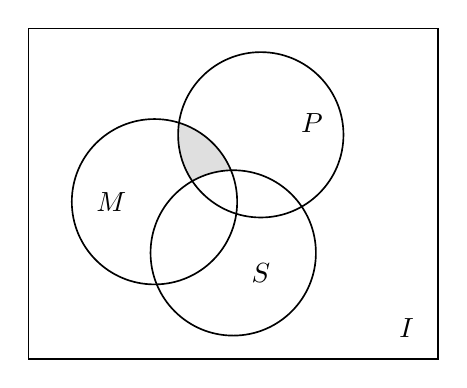
\begin{tikzpicture}[line width=.6pt,font=\normalsize]
\draw (-2.6,-2.1) rectangle (2.6,2.1);
\begin{scope}
\clip (-1.0,-0.1) circle (1.05);
\clip (0.35,0.75) circle (1.05);
\fill[gray!25] (-2.6,-2.1) rectangle (2.6,2.1);
\end{scope}
\begin{scope}
\clip (-1.0,-0.1) circle (1.05);
\clip (0.35,0.75) circle (1.05);
\clip (0.0,-0.75) circle (1.05);
\fill[white] (-2.6,-2.1) rectangle (2.6,2.1);
\end{scope}
\draw (-1.0,-0.1) circle (1.05);
\draw (0.35,0.75) circle (1.05);
\draw (0.0,-0.75) circle (1.05);
\node at (-1.55,-0.1) {$M$};
\node at (1.0,0.9) {$P$};
\node at (0.35,-1.0) {$S$};
\node at (2.2,-1.7) {$I$};
\end{tikzpicture}
